% !TEX root = ..\main.tex
\chapter{State-of-the-Art}

This chapter presentes the state-of-the-art topics which is relevant to this project. Section 2.1 looks into technical debt with its definitions, types etc. Section 2.2 looks into embedded systems and some of the challenges with it. Section 2.3 presents 


\section{Technical Debt}


A developer has the choice to implement a functionality in two different ways. The first one is a less good solution, known as the "quick and dirty" way\cite{p29-cunningham}. The developer will deliver the functionality in time, but we trade off design and quality, which makes operation, management and maintenance hard to do. The other choice is a much cleaner result, but in exhange of more time to put the functionality in place. This choice also makes changes and implementations of new functionality a lot easier in the future\cite{url-fowler}. This is what technical debt is, when shortcuts trading of design and quality in order to solve a problem in time. The concept of technical debt was first introduced by Ward Cunningham in 1992 in order to communicate the problem with non-technical stakeholders\cite{p29-cunningham}. He defines the term in terms of low quality code. 

Technical debt is a big problem today. In 2010, the total debt was around 500 millions dollar, while it's estimated that in 2015 the technical debt will be around 1 billion dollar\cite{gartner2010}.


\subsection{Comparation with financial debt}
Techincal debt has many similarities as financial debt, which can be seen as the following:
\begin{itemize}
	\item You take a loan that has to be repaid later
	\item You usually repay the loan with interest
	\item If you can't pay back, a very high cost will follow. For example, you can loose your house or car.
\end{itemize}

Just like financial debt, technical debt needs to be repaid with interests\cite{wiki:techdebt}. If the debt is not repaid, local maintenance will be hard, and it may lead to software project failure - the customer gives up and goes somewhere else, the system has to be rewritten, or collapse of the company. 

However, there are some differences as well. The debt has to be repaid eventually, but not on any fixed schedule. This means that some debts may never have to be paid back, which depends on the interest and the cost of paying back the debt. The person who takes the debt is not necessaryly the one who has to pay it off. A software project which moves from development mode to maintencance mode might change the engineers as well. So the engineers who has to maintain the system are the one who has to pay back the debt which occured in the development mode. Developers are often rewarded for their implementation speed. However, technical debt is not about bad code design. In practice, it's much more than that. Example on interests might be lowr pace of development, low competitiveness, security flaws on the system, loss of developers and their expertise, poor internal collaboration environment, dissatisfied customers and loss of market share\cite{p50-allman}.


Til forskjell fra finansiell gjeld kan teknisk gjeld aldri betales tilbake i sitt fulle. Å betale TG kommer i en form av hvor lang tid det tar å fikse koden/problemet. Men det er ikke lett å vise hvilke gjeld som har høyest kost. Er interessen lavere enn hva det koster, er det ikke vits i å betale tilbake. Eksempel: Man har et system som trenger en oppgradering som kan koste 1 million. Man tar valget i å ikke oppgradere, og satse på at systemet fungerer. Det gjør det ikke, systemet går ned og firmaet taper felre millioner på å reparere systemet. Her kunne man spart penger på å oppgradere.



\subsection{Types of technical debt}

McConnels defines two categories based on how they are incurred, intentionally or unintentionally. The unintentional category includes debt that comes from doing a poor job. For instance, uninntentional debt might be when a junior software developer writes bad code due to lack of knowledge and experience. Intentional debt occurs when an organization makes a decision to optimize for the present rather than the future. An example is when the project release must be done on time, or else there wont be a next release. This leads to bad decisions, like taking a shortcut to solve a problem, and reconcile the problem after shipment

Fowlers presents a formal explanation of how techincal debt can occur. He categories technical debt into different debt types, in which he calls "Technical Debt Quadrant". As seen in the figure, the debt is grouped into four categories: reckless deliberate/inadvertent and prudent deliberate/inadvertent. Reckless-deliberate is descibed as "we dont have time for design", while reckless-inadveretnt is described as "waht's layering?". Prudent-deliberate is described as "we must ship now and deal with the consequences" and prudent-inadvertent is described as "now we know what we should have done". Figure \ref{fig:techDebtQuad} shows the following quadrant.

\begin{figure}
	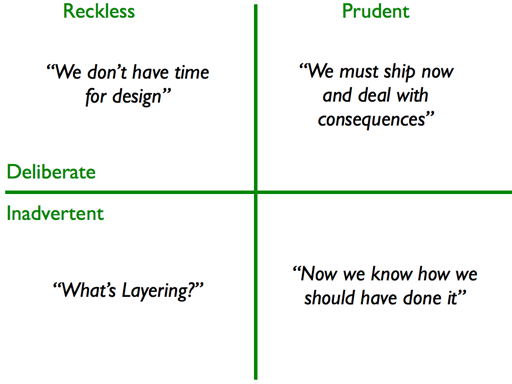
\includegraphics[width=0.8\textwidth]{images/techDebtQuadrant.png}
	\caption{Technical Debt Quadrant}
	\label{fig:techDebtQuad}
\end{figure}

Krutchen divides technical debt into two categories\cite{krutchen}. Visible, debt that is visible for everyone. It containts elements such as new functionality to add and defects to fix. Invisible is the other category, debt that is only visible to software developers.

\subsection{Organizational debt}
While technical debt is known problem, there's one more type of debt which can be accrued on a compandy-wide level. This type of debt is called organizational debt. Organizational debt is all about people and culture compromises made to "just get it done" in early stages of a startup\cite{steve-blank}.  

Technical debt is issues within the software which hampers its maintenance, which leads to that organizational debt is issues preventing a company from running smoothly. When things should be going great, organizational debt can turn a growing company to a nightmare. Growing companies needs to know how to recognize and refactor organizational debt. 

Reasons for technical debt:

\begin{itemize}
	\item Training the new hires, both culture and specific tasks
	\item Retain existing hire by doing something for them. Many doesn't get promoted. New hire might get a better posistion than existing hire who has been there from the start.
\end{itemize}

Good building, furniture, and compensation for executive staff isnt enough. Think about existing employees who's been there from the start. You might end up loosing qualified people who's spent years building up the company, but not compensated for it. Top-down approach is focused too much. Think about the bottom employees.They have the inistituinal knowledge and hard-earned skills.

When new people got hired, the ones who could train them about the company culture and how to do their specific tasks is the old employees who's being underpaid. They will look for another job. No one would be able to train the new people then. Giving compensation in form of stock vesting, insurance benefits, movie nights etc isnt enough as everyone gets it. Do something for the employees who's been there for a long time.

Refarocting might be important in order to reduce the organizational debt. Write plan for managing new wave of hires before hiring them. Sometimes, you'll also need to think about what you will have to do if you're about to loose a key employee. Is it worth to replace employees who hold critical knowledge? Put together an expence budget using the current employee salaries. See who's important. Identify the one they wanted to keep and upgrade them. Some employees might not be that important as welll as they might be a performance problem for the whole organization. Need to look at the company culture as well, does it take into account of the new size and stage of the organization? What have the company achieved, what are the key elements that have made it great so farm, are they same of different. Think about the customer too. Does we talk to the customer, or does the customer talk to us. Also, keep in mind that an adivosory board of other CEOS who've been through the early stages might be good. Failure to refactor might kill a growing company\cite{steveblank}.

Some examples on organizational debt:
\begin{itemize}
	\item Different departments solving the same problems might use differnet methologies and tools. Difficult to see similarities in order to address company-wide issues.
	\item Creation of processes and implement solutions which seems great at first, but didnt address the root casue of the issue and ending up creating more problems.
	\item Time constraints, solving a problem in less-than-ideal manner this time. This manner is repeated because no one remember that the first time was intended to be one-off situation.
\end{itemize}


\subsection{Why does it occur}
Many thinks that technical debt is mostly related to code decide. However, technical debt might occur already in the requirement specification phase in software development project. 

Technical debt may be caused by several factors:
\begin{itemize}
	\item Work processes: Software development methology, can some tasks be automized (with a deploy script), is tests written after bug fixing, do you map and document shortcuts you take, is there any plans for techincal debt management later, is it important to implement new functionality or to make sure that the existing ones work propertly?
	\item People (knowledge and capacity): Do you need some individuals to finish a task, Do you have the right people for the job, is enough training given to new people, what happens if you need someone who's on vacation/change project/is sick or something. You should keep this in mind and make a plan on how knowledge is transferred. Techcnical debt can be the reason for poor motivation and productivity which causes you to work poorly. 
	\item Technology: Is solutions hard to integrate with other solutions, is all the systems out there compatible with newer technology, is there any outdated or duplicated code in the system, is all the systems secure, is the solutions old, or user friendly, is there some code which is hard to maintencance. 
	\item Collaboration in the organization: Commuinication between developers and requirement people. You often get a list with requirements, is the list understandable? Do we work with a backlog with tasks that should have been solved long time ago, but not which is not "actual" now?
\end{itemize}
Developers might not care about the product because they don't feel that they "own" what's being made. They get told what do to, but not more than that. Can't make requirements.


Operating technical debt might be to maintenance and manage existing code rather than implementing new functionality. It is important to keep track of the technical debt, and incur interest payments, before it makes troubles for you. Do do that, you could for example set up a plan for repayment which tells you something about how the debt shall be repayed. Scrum can be used to do this for example, where you split the repayment plan to smaller parts where you estimate and prioritize tasks. It is important to remember that taking too much loan might cause problems. As mentioned ealier, technical debt can be seen as taking a financial loan according to Cunningham. The loan has to be repaid with interests. Technical debt uses time and effort as repayment. It is acceptable to take a loan, but it should be controlled. Do not take loan than what you are able to handle. Think with your head.


Når det kommer til teknisk gjeld er det ikke alltid personen som har utviklet noe som tar ansvar, men kan en annen kan ta seg av den gjelda. Mange utviklere vedlikeholder ikke sin egen kode. Mange selskaper har også regler om at når et software er ferdig utviklet av de "beste" til å bli vedlikeholdt av de nest beste, som ofte kan få mindre betalt men har mye mer arbeid å gjøre. Ingen i din organisasjonen viser interesse for det, er brukerne som må betale for gjelda. Utviklere er belønnet for hvor raskt de implementerer enn langsiktig vedlikehold og kan ha fått seg et nytt prosjekt før gjelda er betalt. Få systemer har TODO eller FIXME kommentarer i kildekoden. 




\subsection{Technical debt in Industry}
Technical debt today is connected with many differnet aspects in the software development process, like documentation debt, requirements debt, architecture debt etc. 

Using sequential design processes in software development processes to build complex, intensive systems is often a failure. Requirements are specified at the beginning of the software development process, and the remaining software development activities has to follow the initiral requirements. This kind of model is not appropiate to use for big softwares where technology and business requirements always change. This is why agile methods was made, where change and feedback is important. One of the benefits is the ability to quickly release new functionality. However, one of the problems with agile methods is that developers often wants to focus on implementing new fucntionality, which results in poor focus on design, code quality, testing, which again leads to technical debt.  

Klinger carried out an industrial case study at IBM where four technical architechts with different backgrounds were interviewed and the goal was to examine how the decisions to incur debt was taken and the extend to which the debt provided leverage\cite{p35-klinger}. What they found out was that the company failed to assess the impact of intentionally incurring debt on projects. Decisions regarding technical debt were rarely quantified. There were also big organizational gaps among the business, operational and technical stakeholders, which incurred debt.

Codabux carried out an industrial case study where the topic was agile development focusing on techincal debt\cite{p8-codabux}. They wanted to gain insights on agile adoption and how techincal debt affects the development processes. This industiral case study happened in form of an interview. After conducting the research, they got two definitions of technical debt, further known as infrastructure and automation debt. Infrastrucutre is the work that improves the teams processes and ability to produce a quality procudt with refactoring, repackaging, developing unit tests. Automation isthe work relatedd to supporting continious integration and faster development cycles. The term technical debt was mostly related to design, testing and defect debts according to the participants. One of the engineers mentioned that when they were working, they didn't know the "balacne of the credit card. They kept charging it". Management decides when enough debt has incurred, and is influenced by the customer needs.







%%%%%%%%%%%%%%%%%%%%%%%%%%%%%%%%%%%%%%%%%%%%%%%%%%%%%%%%%%%%%%%%%%%%%%%%%%%%%%%%%%%%%%




\section{Embedded Systems}
With the rapid evolution of electrical and software based systems, known as embedded systems, we see that most of the future compuing systems will be embedded systems\cite{wolfmadsen-2000}. However, as the complexity of embedded systems increases, maintaining the quality of such systems becomes more difficult. Higher functionality is provided when multiple components are combined together with embedde systems. This type of combination leads to higher cost of verifying additional software, which makes many fail to test the product properly and deliver reliable products. Companies must often recall their products, and catching these software defects earlier in the system design process saves a lot of money. The ability to identify these kind of problems earlier is still something many companies has troubles with. Embedded systems has also long lifetime and it's important to find out how to make decisions so future maintenance and operation has low cost as possible. Technical debt is a big factor in embedded systems as developers might not be available years after implementaion. 

Since embedded systems are some specialized hardware,


\subsection{Embedded system software}

Embedded software is a computer software for embedded systems. It is specialized for a type of hardware which it lays and runs on. Therefore, embedded software might have multiple constraints related to run-time, memory usage, processing power etc.

 
Embedded software had an important role today with the rapid evolution of ES. Escpecially with the Internet of Things trend.

However, there are some challenges with embedde system software. These type of software usually has long lifetime. Old systems are usually hard to maintain compared to new ones. Companies must maintain many different configurations, and maintaining systems are challenging due to time. It is important to take the right choices when designing such systems. Abstract and high level design, architecture. People tend to deliver something in time rather than making something good. 


\subsection{Virtualization of embedded systems}


\section{Configuration management}

Dart defines configuration management as a dicipline for controlling the evolution of software systems (siter dart). This includes content, changes and status in a shared project. Both processes and technical solutions to handle changes and the projects integrity. Example, if a new version of the product is released, everything related to this projects needs to be up-to-date. Like documentation. Configuration management identifies every component in a project and has an overview of every suggestions and changes from day 1 to the end of the product.

Software CM is a dicipline for controlling the evolution of software systems. Some examples on SCM is Git-SCM, SVN, RCS, Adele, ClearCase. Version control is the key behind SCM. IEEE standard 729-1983 highlights the following operational aspects of CM:

\begin{itemize}

	\item \textbf{Idenfitication}: The products structure. Identifies every component in the products, making them unique and accessible in some form.
	\item \textbf{Control}: Controls every reelase and changes of a product throghout the lifecycles by having some controls in place that ensure consistent software via the creation of ab aseline product.
	\item \textbf{Status accounting}: Records and reports the status of components and change requests. It is also possible to review statistics about components in the product.
	\item \textbf{Audit and review}: Validates the product and maintaining the consistency between components by ensuring that the product is a well-defined collection of compontens.
\end{itemize}

In addition th those aspect, we can expect the definition of CM by three more aspects
\begin{itemize}
	\item \textbf{Manufacture}: Maintaining the construction, and build the product in an optimal way.
	\item \textbf{Process management}: Take care of the companies policies, processes and lifecycle model.
	\item \textbf{Teamwork}: Review the work and make sure that the collaboration is good. Keep an eye on the interaction between multiple users and the product.

\end{itemize}

When do we use CM? 



Når skal CM brukes? Det varierer. Noen velger å bruke CM system når produktet har gått gjennom utviklingsfasen og er klar for lansering/shipment. Andre velger å putte alt i CM ved oppstart av prosjektet. Begge har sine overheads. Man kan ta et valgt basert på overheads ved en endring. Er det mye manuell arbeid som å fylle ut diverse former, søke om godkjennelse osv vil man ofte plassere programverer under CM etter utvikling. Men hvis en forespørslen om en endring bruker lite tid og innsats fra utviklere, kan man velge å implementere tidlig. I teorien kan CM implementeres i alle stadiger i produktets livssyklus som opprettelse, utvikling, release, levering til kunde, bruk av produkt osv. Men ideelt sett bør et CM ha lite overhead som mulig, slik at software til CM implementeres så tidlig som mulig. Eksisterende CM systemer fokusterer dessverre på en viss fase i livsfasen, så brukere er begrenset av funksjonaliteten.



Ved å velge en robust SCM system gjør det oss mulige til å håndtere store og komplekse filmengder, støtter distribuert utvikling. En riktig kombinasjon av SCM system og "best practices" gjør det mulig for embedded development projects i å progressere raskt og effektivt.


Noen utfordringer med utvikling av embedded systemer er følgende:
-	Complex file sets
o	En embedded system består av flere komponenter, både hardware og software. Dette gjør systemet komplekst siden et slikt system kan ha mange varierte komponenter. Systemer kan også ha ulike varianter av komponenter til en spesifikk platform slik at man kan selge t produkt ved å endre ltit på krav. Å håndtere disse variantene er en stor utfordring. En annen utfordring er at produkter krever en korrekt versjon av en komponent. Å sørge for at korrelasjonen mellom hver komponent og deres avhengige filer er vedlikeholdt er en utfordring det å.
-	Distributed teams
o	Komponenter kan utvikles i ulike steder i vår verden. Samtidig kan to teams to forskjjelige steder jobbe med samme komponent, spesielt når noe outsources. Slikt samarbeid krever at utviklere har adgang til hver andres arbeid. Utfordringen er at utviklere som jobber i hvert sitt sted (geografisk) holder seg synkronisert.
-	Management and versioning of intellectual property
o	Siden embedded systemer ofte tar I bruk tredje-parts teknologier, er det viktig at de utviklerne bak disse teknologiene oppdater og vedlikeholder arbeidet sitt. Disse oppdateringene må også være sporbare slik at prosjektet inneholder riktig, kompatibel og stabil versjon av teknologien. Utfordringen er å tillate disse utviklerne å sjekke inn contributions og spore endringer i det man har kontribuert. Velge man noe open source ervel dette ikke et problem?





\section{Software reuse}
Software reuse is about using existing software artifacts, or knowledge, to create new software, rather than building it from scratch. Software reuse is a key method for improving software quality. 


\section{Software development life cycles} % (fold)






\section{Software maintenance and evolution}
%http://www.cs.uah.edu/~rcoleman/CS499/CourseTopics/IEEE_Std_1219-1998.pdf
http://www.kantega.no/livslop/
http://swreflections.blogspot.no/2011/04/lientz-and-swanson-on-software.html

After the software is transferred to the users, software will enter maintenance mode. Software maintenance according to IEEE 1219 is defined as "modification of a software after delivery to correct faults, to improve performance or other attributes, or to adapt the product to a modified environment." however, the definition is poor defined term and little used in the industry. Most research today has been on the inital development phase. Configuration management has made contributions to software maintenance. 

The term maintenance can also be appliec to the problem of keeping web pages and software applications up to date and consistent.

Lientz and Swanson did a survey back in the 1970s with 487. The survey where they categorized maintenance into four categories:
- Adaptive: Changes in the software environment
- Perfective: New requirements
- Corrective: Fixing errors
- Preventive: Preventing future problems
According to van Vliet, the real maintenance activity corrective maintenance. However, the survey showed that nearly 75 \% of the attendees spent their time on category 1 and 2. Nearly 22 percent on category 3 and 3 percent on category 4. Why didn't they spend more time on fixing bugs and preventing future erros? Most severe maintenance problems was caused by poor documentation, demand from users for changes, difficulty meeting schedulment, problems training new hires.  Some other problem areas was lack of user understand and user training, the customers didnt understand how system works. Programmers had low productivity, skill level and motivation. System was badly designed leading to low quality. How much has this changed since then? it looks like that new user requirements is the main problem for software evolution and maintenance.

Change: According to Viet, perfective consumes 50\%, adaptive consumes \%25, corrective 21 and 4 on 

Software maintenance is important because it consumes a larg part of the lifecycle costs and that if not able to change software quickly to adapt to software environment means that business opportunities are lost.


A model called stage model basded on empirical observation was defined by Bennet and Rajlich. This model helps us analysing maintenance and evolution of software development. Maintenance was seen as a single activity after initial development, however, a staged model was introduced which split maintenance into five distinc stages. The reason is to separate maintenance into an evolution stage followd by servicing and phase out stages. To make this possible, both software architecture and software team knowledge needs to be well made. Architecture needs to be well defines as it will be used for the rest of the life of the program. Knowledge is abhout the knowledge og the app domain, requirements, algorithms, data formats, strength/weaknesses of program/architecture/environment.

Servicing stage is about small changes, usually patches and code changes. The program is not evolvable here. 

Software evolution is a process that usually takes place when the initial development of a software project is done and was successfull. The goal of software evolution is to incorporate new user requirements in the application and adapt it to the existing application. This phase is important beacuse it takes a lage part of the overall lifecycle costs. It is also important because these days technology tend to change rapidly, and not following these trend means loosing business oppertunities.

Final stages are phase out and close-down. System might be in production, but no service is undertaken. During close-down, software is disconnected. 

An amplified of this staged model was defined as well, versioned stage model. The difference between this model and the simple stage model is that during evolution, versions of software are being made. All new functionality or changes are implemented in the future versions. If a version becomes outdated, it is replaced with a new version.	







